\documentclass[../DoAn.tex]{subfiles}
\begin{document}

Chương 4 đã kiểm chứng ngữ nghĩa và phân tích xu hướng hiệu năng của nhóm lệnh mở rộng trên gem5. Từ kết quả mô phỏng đó, bước đánh giá tiếp theo là kiểm tra xem xu hướng tăng tốc có còn giữ trên phần cứng thật hay không, khi các thao tác AI lượng tử hóa được ánh xạ vào chương trình nhúng và sử dụng trong cả các nhân INT8 lẫn mô hình MNIST dạng mạng kết nối đầy đủ chạy trên kit DE2i-150/CV32E40P. Trên cơ sở đó, chương này trình bày nền tảng thực nghiệm, các ràng buộc triển khai về thời gian, bộ nhớ và giao tiếp ngoại vi, phương pháp đo, kết quả với các nhân INT8, kết quả với mô hình AI lượng tử hóa chạy bằng TensorFlow Lite Micro, cùng tài nguyên và kết quả phân tích thời gian của thiết kế sau triển khai.

\section{Nền tảng phần cứng và luồng triển khai trên kit}
\label{sec:nen-tang-phan-cung-kit}

Để chuyển từ mô phỏng sang phép đo trên phần cứng, đồ án xây dựng một SoC tối thiểu trên kit DE2i-150, với FPGA Cyclone IV GX làm môi trường tích hợp và CV32E40P làm lõi RISC-V thực thi chương trình nhúng. Vì CV32E40P chưa bao gồm bộ nhớ và ngoại vi ở mức hệ thống, lõi được kết nối với BRAM, UART và LED để chương trình không hệ điều hành có thể chạy, quan sát trạng thái và trả kết quả đo về máy tính. Trong cấu hình thí nghiệm, tham số \texttt{COREV\_PULP=1} được bật để sử dụng các lệnh CORE-V/PULP cho nhóm thao tác AI lượng tử hóa, đồng thời FPU được tắt vì các bài toán trong đồ án đều dùng suy luận INT8 \cite{openhw_cv32e40p_um_2024}.

Các thông số chính của nền tảng thực nghiệm được tóm tắt trong Bảng~\ref{tab:de2i150-experiment-platform}.

\begin{table}[H]
    \centering
    \footnotesize
    \renewcommand{\arraystretch}{1.00}
    \begin{tabular}{|>{\raggedright\arraybackslash}p{3.45cm}|>{\raggedright\arraybackslash}p{9.20cm}|}
        \hline
        \textbf{Thành phần} & \textbf{Cấu hình sử dụng trong thực nghiệm} \\
        \hline
        Kit và FPGA & Terasic DE2i-150, FPGA Cyclone IV GX \texttt{EP4CGX150DF31C7}. \\
        \hline
        Lõi xử lý & CV32E40P, \texttt{COREV\_PULP=1}, \texttt{COREV\_CLUSTER=0}, \texttt{FPU=0}. \\
        \hline
        Tần số hoạt động & 50 MHz, sử dụng tín hiệu xung nhịp \texttt{clock\_50} của kit. \\
        \hline
        Bộ nhớ cục bộ & BRAM 128 KB tại địa chỉ bắt đầu \texttt{0x00000000}, chia thành bốn làn byte để ánh xạ vào các khối M9K. \\
        \hline
        Giao tiếp ngoại vi & UART TX/RX 115200 8N1 qua vùng vào/ra ánh xạ bộ nhớ tại \texttt{0x02000000}; LED tại \texttt{0x03000000}. \\
        \hline
        Chương trình nhúng & Chương trình không hệ điều hành, biên dịch ở chế độ \texttt{rv32im\_zicsr}; không dùng tập lệnh nén trong giai đoạn đo nhân để giữ thân vòng lặp phần cứng thẳng hàng 32 bit. \\
        \hline
        Đo hiệu năng & Đọc trực tiếp các thanh ghi CSR \texttt{mcycle} và \texttt{minstret}; kết quả và checksum được in qua UART. \\
        \hline
    \end{tabular}
    \caption{Cấu hình nền tảng thực nghiệm trên kit DE2i-150/CV32E40P}
    \label{tab:de2i150-experiment-platform}
\end{table}

Việc giữ nguyên cấu hình phần cứng, tần số hoạt động, bản đồ bộ nhớ và phương thức thu kết quả giúp các phép đo nhân INT8 và mô hình MNIST FC ở các mục sau có cùng điều kiện so sánh.

Từ cấu hình trên, có thể thấy CV32E40P là khối xử lý trung tâm, còn BRAM và các ngoại vi tạo thành môi trường tối thiểu để chương trình có thể chạy và trả kết quả. Ở mức RTL, Hình~\ref{fig:quartus-cv32e40p-core-rtl-view} là ảnh cắt từ RTL Viewer của Quartus sau tổng hợp, cho thấy thực thể CV32E40P cùng các nhóm tín hiệu chính như xung nhịp/khởi tạo lại, giao tiếp lệnh, giao tiếp dữ liệu, ngắt và gỡ lỗi. Hình này được sử dụng để minh họa phần lõi trong thiết kế, trước khi trình bày luồng triển khai đầy đủ ở mức hệ thống.

\begin{figure}[H]
    \centering
    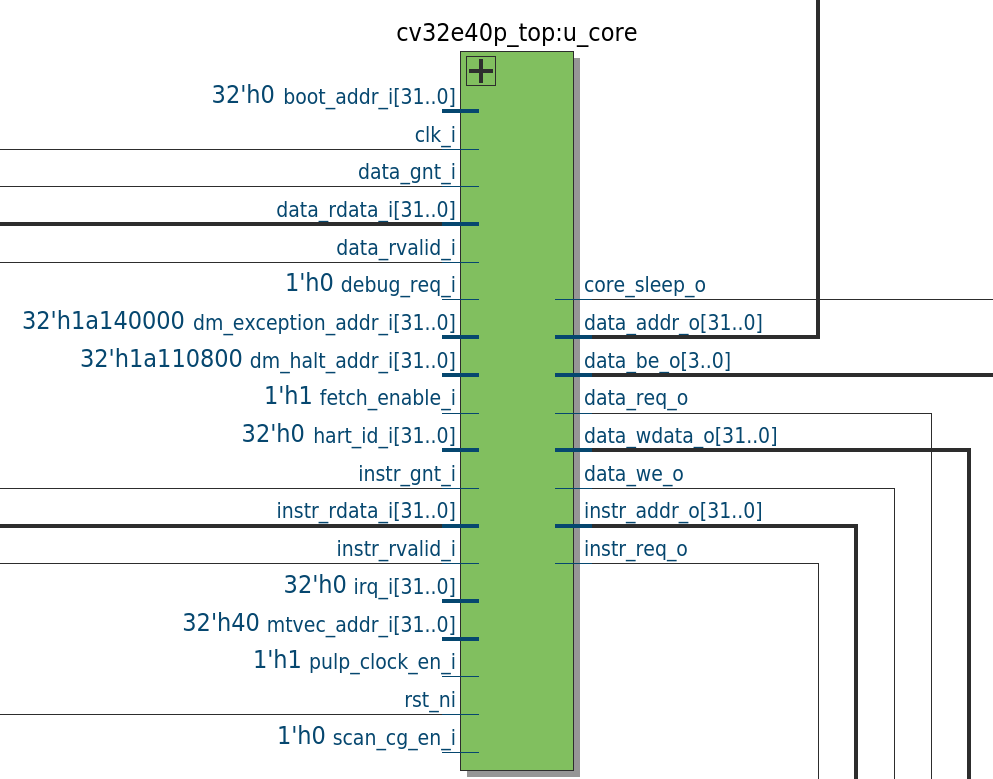
\includegraphics[width=0.8\linewidth]{Hinh_ve/quartus_cv32e40p_core_rtl_view.png}
    \caption{Ảnh cắt RTL Viewer của khối CV32E40P trong thiết kế SoC}
    \label{fig:quartus-cv32e40p-core-rtl-view}
\end{figure}

Bao quanh lõi CV32E40P là module mức đỉnh của SoC. Module này ánh xạ hai cổng OBI của lõi tới BRAM và các ngoại vi vào/ra ánh xạ bộ nhớ. Cổng lệnh chỉ đọc từ BRAM, trong khi cổng dữ liệu có thể đọc/ghi BRAM, truy cập thanh ghi trạng thái UART, ghi byte phát UART, đọc byte nhận UART và cập nhật LED trạng thái. Cách tổ chức này giữ phần cứng ở mức vừa đủ cho mục tiêu đo hiệu năng: chương trình chạy trực tiếp trong BRAM, còn UART đảm nhiệm đường truyền kết quả về máy tính.

Thiết kế không sử dụng bộ nạp chương trình ở thời gian chạy, nên nội dung BRAM được đưa vào FPGA ngay trong quá trình tổng hợp. Chương trình nhúng sau khi biên dịch được chuyển thành bốn tệp hex theo mẫu \texttt{firmware\_byteN.hex}, với \texttt{N} từ 0 đến 3, rồi được Quartus nạp vào các làn byte của BRAM thông qua \texttt{\$readmemh}. Vì vậy, mỗi phiên bản chương trình dùng cho đo nhân hoặc TensorFlow Lite Micro tương ứng với một tệp cấu hình FPGA có nội dung BRAM đã được cố định.

Bên cạnh cấu trúc phần cứng nêu trên, quá trình xây dựng nền tảng còn bao gồm các chỉnh sửa tương thích với Quartus Lite. Cụ thể, đồ án lựa chọn các tệp RTL cần thiết, thay khối điều khiển cổng xung nhịp dùng cho mô phỏng bằng phiên bản phù hợp với FPGA, chuyển một số cú pháp SystemVerilog-2012 sang dạng SystemVerilog-2005 mà Quartus chấp nhận, viết module mức đỉnh của SoC bằng Verilog-2001 và kiểm tra các chương trình nhúng cơ bản. Các chỉnh sửa này thuộc giai đoạn đưa CV32E40P lên FPGA ban đầu; những thay đổi liên quan tới bật PULP, xử lý ràng buộc thời gian và đo hiệu năng được trình bày riêng ở các mục tiếp theo.

Trên nền tảng đã được cố định đó, các thí nghiệm trong chương này được triển khai theo cùng một luồng, như khái quát trong Hình~\ref{fig:de2i150-soc-experiment-flow}. Trên máy tính điều khiển, chương trình nhúng được biên dịch bằng bộ công cụ RISC-V và chuyển thành các tệp hex theo từng làn byte để khởi tạo BRAM. Quartus tiếp đó tổng hợp thiết kế, tạo tệp cấu hình FPGA và nạp xuống kit. Khi chương trình bắt đầu chạy, CV32E40P thực thi mã lệnh trong BRAM, truy cập UART/LED qua vùng vào/ra ánh xạ bộ nhớ và gửi kết quả đo về máy tính. Sơ đồ này tập trung vào các quan hệ chức năng cần thiết cho quá trình đo, trong khi các chi tiết tín hiệu mức RTL được lược bỏ để giữ mạch trình bày ở mức hệ thống.

\begin{figure}[H]
    \centering
    \resizebox{0.96\linewidth}{!}{\begin{tikzpicture}[
    font=\scriptsize,
    block/.style={draw, rounded corners=2pt, align=center, minimum height=0.92cm, fill=gray!8},
    host/.style={block, text width=3.25cm, fill=yellow!15},
    flow/.style={block, text width=3.25cm, fill=orange!10},
    core/.style={block, text width=3.10cm, fill=blue!8},
    mem/.style={block, text width=3.10cm, fill=purple!10},
    io/.style={block, text width=2.65cm, fill=cyan!8},
    note/.style={align=center, font=\scriptsize\bfseries},
    arrow/.style={-{Latex[length=2mm]}, thick},
    bus/.style={<->, >=Latex, thick},
    serial/.style={-{Latex[length=2mm]}, thick, densely dashed}
]
    \node[host] (host) at (-5.35, 1.10) {Host PC\\RISC-V toolchain\\Quartus};
    \node[flow] (hex) at (-5.35, -1.10) {Firmware\\\texttt{.elf/.bin}\\byte-lane hex};

    \node[note] at (2.30, 2.65) {DE2i-150/CV32E40P SoC trên FPGA};
    \draw[rounded corners=3pt, thick, fill=green!4]
        (-1.65, -2.05) rectangle (6.25, 2.25);

    \node[core] (core) at (0.35, 0.75) {CV32E40P\\\texttt{COREV\_PULP=1}\\\texttt{FPU=0}};
    \node[mem] (bram) at (0.35, -1.05) {BRAM 128 KB\\4 byte-lane M9K\\\texttt{\$readmemh}};
    \node[io] (uart) at (4.40, 0.75) {UART TX/RX\\115200 8N1};
    \node[io] (led) at (4.40, -1.05) {LED status\\heartbeat};

    \draw[arrow] (host) -- node[right, xshift=0.06cm] {build} (hex);
    \draw[arrow] (hex.east) -- node[above, pos=0.55] {BRAM init} (bram.west);
    \draw[bus] (core.south) -- node[right] {OBI I/D} (bram.north);
    \draw[bus] (core.east) -- node[above] {MMIO} (uart.west);
    \draw[arrow] (core.east) -- ++(0.55,0) |- node[pos=0.70, below] {MMIO} (led.west);
    \draw[serial] (uart.north) .. controls (3.55,2.45) and (-2.75,2.35) ..
        (host.north east);
\end{tikzpicture}
}
    \caption{Luồng triển khai và thu kết quả thực nghiệm trên kit DE2i-150/CV32E40P}
    \label{fig:de2i150-soc-experiment-flow}
\end{figure}

\section{Hiện thực CV32E40P/PULP trên FPGA và xử lý ràng buộc thời gian}
\label{sec:cv32e40p-pulp-timing}

Trên nền tảng SoC đã mô tả ở Mục~\ref{sec:nen-tang-phan-cung-kit}, bước tiếp theo là cấu hình lõi CV32E40P để sử dụng nhóm lệnh CORE-V/PULP. Đây là lựa chọn phù hợp với mục tiêu thực nghiệm của đồ án: lớp thao tác đã đặc tả ở Chương~\ref{chap:de-xuat} được hiện thực bằng cách ánh xạ sang các đơn vị thực thi mở rộng trong CV32E40P, gồm ALU/MUL mở rộng, nhân tích vô hướng trên dữ liệu đóng gói, tải/lưu hậu tăng và vòng lặp phần cứng \cite{openhw_cv32e40p_um_2024}. Trọng tâm công việc vì vậy không chỉ nằm ở việc bật cấu hình PULP, mà còn ở quá trình đưa cấu hình này qua luồng tổng hợp FPGA, xử lý các ràng buộc thời gian phát sinh và xây dựng firmware để gọi đúng ngữ nghĩa của các thao tác \texttt{mac}, \texttt{dot4\_acc}, \texttt{p.lw} và \texttt{lp.setup} trên phần cứng thật.

Việc bật \texttt{COREV\_PULP=1} đồng thời làm đường dữ liệu trong lõi phức tạp hơn, đặc biệt ở các đường chuyển tiếp toán hạng giữa các tầng của đường ống lệnh. Trong lần tổng hợp ban đầu trên Cyclone IV, thiết kế sau bước đặt và định tuyến chỉ đạt \(F_{\max}\) xấp xỉ \(37{,}6\,\mathrm{MHz}\), thấp hơn tần số mục tiêu \(50\,\mathrm{MHz}\) của kit. Đường giới hạn không nằm ở UART hay BRAM, mà nằm ở phụ thuộc dữ liệu trực tiếp giữa hai lệnh ALU/MUL liên tiếp: kết quả vừa sinh ra ở tầng EX phải đi qua mux chuyển tiếp ở tầng ID rồi được chốt vào thanh ghi toán hạng ID/EX trong cùng một chu kỳ. Đường tổ hợp này được khái quát ở Hình~\ref{fig:fpga-timing-bubble}.

\begin{figure}[H]
    \centering
    \resizebox{0.96\linewidth}{!}{\begin{tikzpicture}[
    font=\scriptsize,
    stage/.style={draw, align=center, minimum width=1.05cm, minimum height=0.58cm, fill=gray!10},
    exstage/.style={stage, fill=blue!10},
    idstall/.style={stage, dashed, fill=cyan!12},
    inst/.style={anchor=east, font=\ttfamily\scriptsize},
    note/.style={align=center, font=\scriptsize},
    dep/.style={-{Latex[length=2mm]}, very thick, red!75},
    okpath/.style={-{Latex[length=2mm]}, thick, blue!75},
    flow/.style={-{Latex[length=1.8mm]}, thick, gray!70},
    stallarrow/.style={-{Latex[length=1.8mm]}, thick, orange!85!black}
]
    \foreach \x/\c in {0/C1,1.70/C2,3.40/C3,5.10/C4,6.80/C5,8.50/C6} {
        \node[note, text width=1.0cm] at (\x, 1.88) {\c};
        \draw[gray!35] (\x, 1.58) -- (\x, -1.92);
    }

    \node[inst] at (-0.40, 0.98)
        {cv.mac x10,x11,x12};
    \node[stage] (mac_if) at (0, 0.98) {IF};
    \node[stage] (mac_id) at (1.70, 0.98) {ID};
    \node[exstage] (mac_ex) at (3.40, 0.98) {EX\\sinh x10};
    \node[stage] (mac_wb) at (5.10, 0.98) {WB\\ghi x10};

    \node[inst] at (-0.40, -1.02)
        {add x13,x10,x14};
    \node[stage] (add_if) at (1.70, -1.02) {IF};
    \node[idstall] (add_id0) at (3.40, -1.02) {ID\\đọc x10};
    \node[idstall, fill=orange!12] (add_id1) at (5.10, -1.02) {ID giữ\\EX rỗng};
    \node[exstage] (add_ex) at (6.80, -1.02) {EX};
    \node[stage] (add_wb) at (8.50, -1.02) {WB};

    \draw[flow] (mac_if) -- (mac_id);
    \draw[flow] (mac_id) -- (mac_ex);
    \draw[flow] (mac_ex) -- (mac_wb);

    \draw[flow] (add_if) -- (add_id0);
    \draw[stallarrow] (add_id0.east) -- (add_id1.west);
    \draw[flow] (add_id1) -- (add_ex);
    \draw[flow] (add_ex) -- (add_wb);

    \draw[dep] (mac_ex.south) -- node[left, align=right, text=red!75!black]
        {đường dài\\EX-to-ID} (add_id0.north);
    \draw[okpath] (mac_wb.south) -- node[right, align=left, text=blue!75!black]
        {đọc từ\\WB/RF} (add_id1.north);
\end{tikzpicture}
}
    \caption{Minh họa chèn một chu kỳ rỗng giữa hai lệnh phụ thuộc dữ liệu trực tiếp}
    \label{fig:fpga-timing-bubble}
\end{figure}

Để phá đường ràng buộc thời gian này, đồ án bổ sung tham số \texttt{FPGA\allowbreak\_TIMING\allowbreak\_MODE} trong bản sao cục bộ của lõi. Khi tham số này được bật, bộ điều khiển phát hiện trường hợp lệnh ở ID đang đọc đúng thanh ghi đích do lệnh ALU/MUL ở EX sinh ra. Thay vì cho lệnh tiêu thụ nhận trực tiếp dữ liệu qua đường EX-to-ID, bộ điều khiển giữ lệnh đó ở ID thêm một chu kỳ, vô hiệu hóa các tín hiệu ghi điều khiển của chu kỳ hiện tại và đưa một chu kỳ rỗng (bubble) vào đường ống lệnh. Sang chu kỳ tiếp theo, kết quả của lệnh sinh dữ liệu đã đi qua đường ghi lại hoặc đường chuyển tiếp từ WB, nên lệnh tiêu thụ có thể đọc toán hạng qua đường ngắn hơn. Tương ứng với thay đổi này, đường chuyển tiếp trực tiếp EX-to-ID bị tắt trong chế độ \texttt{FPGA\allowbreak\_TIMING\allowbreak\_MODE=1}, còn các đường chuyển tiếp khác như WB-to-ID vẫn được giữ.

Điều chỉnh trên là một đánh đổi giữa hiệu năng vi kiến trúc và khả năng đáp ứng ràng buộc thời gian trên FPGA: một số cặp lệnh phụ thuộc trực tiếp có thể mất thêm một chu kỳ, nhưng đổi lại thiết kế đạt được xung nhịp mục tiêu \(50\,\mathrm{MHz}\) trên kit DE2i-150. Vì vậy, các kết quả tăng tốc trong những mục sau được hiểu là số liệu thực nghiệm của cấu hình đã tổng hợp và chạy ổn định trên FPGA, thay vì là ước lượng lý tưởng tách rời khỏi điều kiện triển khai thực tế.

\section{Ánh xạ và kiểm thử smoke nhóm lệnh mở rộng}
\label{sec:anh-xa-smoke-board}

Sau khi cấu hình PULP và xử lý ràng buộc thời gian, bước tiếp theo là bảo đảm rằng các thao tác đã đặc tả ở Chương~\ref{chap:de-xuat} được gọi đúng trên chương trình nhúng. Điểm cần phân biệt là nhánh phần cứng không sử dụng các mã lệnh thử nghiệm trong vùng \texttt{custom-0} như nhánh gem5. Thay vào đó, phần mềm nhúng ánh xạ cùng lớp ngữ nghĩa sang các lệnh CORE-V/PULP của CV32E40P thông qua các hàm bao C/hợp ngữ. Cách tổ chức này giữ giao diện ở mức thao tác gần với đặc tả, trong khi mã lệnh phát ra vẫn phù hợp với phần cứng thật của lõi.

Bảng~\ref{tab:board-ai-op-mapping} tóm tắt lớp ánh xạ được sử dụng trong phần mềm nhúng. Do bộ công cụ RISC-V dùng trong giai đoạn triển khai chưa nhận trực tiếp các tên lệnh CORE-V/PULP dạng gợi nhớ, các hàm bao phát lệnh bằng chỉ thị \texttt{.insn} của trình hợp dịch GNU. Các mã hóa cụ thể được đặt tập trung trong tệp \texttt{ai\_ops.h} của thư mục \texttt{firmware}, nhờ đó các chương trình kiểm thử smoke, bài đo hiệu năng và mô hình suy luận có thể gọi cùng một giao diện hàm.

\begin{table}[H]
    \centering
    \footnotesize
    \setlength{\tabcolsep}{5pt}
    \renewcommand{\arraystretch}{1.24}
    \begin{tabular}{|>{\raggedright\arraybackslash}p{1.95cm}|>{\raggedright\arraybackslash}p{6.25cm}|>{\raggedright\arraybackslash}p{4.35cm}|}
        \hline
        \textbf{Thao tác} & \textbf{Hàm bao trong phần mềm nhúng} & \textbf{Lệnh CORE-V/PULP tương ứng} \\
        \hline
        \texttt{mac} & \texttt{ai\_mac(acc,a,b)} & \texttt{cv.mac} \\
        \hline
        \texttt{dot4\_acc} & \texttt{ai\_dot4\_acc(acc,a,b)} & \texttt{cv.sdotsp.b} \\
        \hline
        \texttt{relu} & \texttt{ai\_relu(x)} & \texttt{cv.max x,x,x0} \\
        \hline
        \texttt{clamp} & \texttt{ai\_clamp(x,ub)} & \texttt{cv.clipur} \\
        \hline
        \texttt{p.lw} & \texttt{AI\_PLW\_U32(ptr,imm)} & \texttt{cv.lw rd,(rs1),imm} \\
        \hline
        \texttt{lp.setup} & \texttt{AI\_LP\_SETUP\_L0(count,body)} & \texttt{cv.setup L0,rs1,uimmL} \\
        \hline
    \end{tabular}
    \caption{Ánh xạ thao tác AI lượng tử hóa sang lệnh CORE-V/PULP}
    \label{tab:board-ai-op-mapping}
\end{table}

Trong bảng trên, hai chi tiết ngữ nghĩa được giữ thống nhất với hành vi thực tế của CORE-V/PULP. Thứ nhất, \texttt{ai\_clamp} giới hạn giá trị về đoạn \([0,ub]\), trong đó cận trên được truyền qua thanh ghi. Thứ hai, \texttt{AI\_PLW\_U32} thực hiện đúng thứ tự tải trước, cập nhật con trỏ sau; vì vậy nếu cần đọc theo một độ lệch cố định, phần mềm nhúng phải điều chỉnh con trỏ trước khi vào vòng lặp. Với \texttt{cv.setup}, trường hằng khi phát bằng \texttt{.insn} không phải là số byte trực tiếp của thân vòng lặp, mà được quy đổi từ số lệnh 32 bit trong thân vòng lặp. Quy ước này được đóng gói trong macro \texttt{AI\_LP\_SETUP\_L0} để tránh lặp lại phép tính khi viết các nhân đo hiệu năng.

Trước khi dùng các lệnh trên để đo hiệu năng, chương trình kiểm thử smoke được xây dựng để kiểm tra từng thao tác một cách độc lập. Kết quả kiểm thử được đưa ra LED đỏ của kit, giúp xác nhận chức năng ngay cả khi chưa dùng UART để in số liệu. Nếu toàn bộ kiểm thử đạt, \texttt{LEDR[7:0]} nhấp nháy giữa \texttt{0xA5} và \texttt{0x00}; nếu một thao tác lỗi, chương trình trả về mã lỗi tương ứng như Bảng~\ref{tab:pulp-smoke-tests}.

\begin{table}[H]
    \centering
    \footnotesize
    \renewcommand{\arraystretch}{1.10}
    \begin{tabular}{|>{\centering\arraybackslash}p{1.55cm}|>{\raggedright\arraybackslash}p{3.40cm}|>{\raggedright\arraybackslash}p{7.55cm}|}
        \hline
        \textbf{Mã LED} & \textbf{Thao tác kiểm thử} & \textbf{Nội dung xác nhận chính} \\
        \hline
        \texttt{0xE1} & \texttt{ai\_mac} & Kiểm tra phép nhân--cộng tích lũy có dấu, chuỗi cộng dồn nhiều lần và trường hợp toán hạng bằng 0. \\
        \hline
        \texttt{0xE2} & \texttt{ai\_dot4\_acc} & Kiểm tra tích vô hướng bốn phần tử INT8 có dấu, được đóng gói trong một thanh ghi, với dữ liệu dương, âm và giá trị biên. \\
        \hline
        \texttt{0xE3} & \texttt{ai\_relu} & Kiểm tra giá trị âm được đưa về 0, giá trị dương được giữ nguyên và trường hợp đầu vào bằng 0. \\
        \hline
        \texttt{0xE4} & \texttt{ai\_clamp} & Kiểm tra chặn dưới tại 0, chặn trên tại \texttt{ub} và các điểm biên như \(x=0\), \(x=ub\). \\
        \hline
        \texttt{0xE5} & \texttt{AI\_PLW\_U32} & Kiểm tra thứ tự tải trước rồi cập nhật con trỏ với các bước \(+4\), \(-4\) và \(+8\) byte. \\
        \hline
        \texttt{0xE6} & \texttt{AI\_LP\_SETUP\_L0} & Kiểm tra vòng lặp phần cứng L0 với thân vòng lặp gồm ba lệnh 32 bit và nhiều giá trị bộ đếm lặp. \\
        \hline
        \texttt{0xA5} & Tất cả kiểm thử đạt & Phần mềm nhúng đã xác nhận sáu thao tác ánh xạ hoạt động đúng trên cấu hình CV32E40P/PULP đang chạy trên kit. \\
        \hline
    \end{tabular}
    \caption{Mã trạng thái LED của chương trình kiểm thử smoke cho nhóm lệnh ánh xạ}
    \label{tab:pulp-smoke-tests}
\end{table}

Như vậy, kiểm thử smoke đóng vai trò là lớp kiểm chứng chức năng trước khi chuyển sang đo hiệu năng. Nhờ bước này, các kết quả ở những mục sau được đặt trên một nền tảng đã được xác nhận: lệnh CORE-V/PULP được phát sinh đúng qua \texttt{.insn}, ngữ nghĩa của từng thao tác khớp với đặc tả của đồ án, và trạng thái LED trên kit cho phép phát hiện sớm lỗi ánh xạ trước khi phân tích các bài đo hiệu năng.

\section{Phương pháp đo và kiểm chứng kết quả}
\label{sec:phuong-phap-do-board}

Sau khi các lệnh ánh xạ đã vượt qua kiểm thử chức năng, bước đo hiệu năng được tổ chức sao cho mỗi kết quả đều có cùng ba thành phần: khoảng đo rõ ràng, mốc so sánh tương ứng và điều kiện kiểm chứng đúng/sai. Toàn bộ chương trình đo chạy trực tiếp trên CV32E40P ở xung nhịp \(50\,\mathrm{MHz}\); máy tính chủ chỉ nhận kết quả qua UART và không nằm trong khoảng đo. Nhờ vậy, các số liệu chu kỳ phản ánh thời gian thực thi trên phần cứng của kit thay vì thời gian giao tiếp với máy tính.

Trong phần mềm nhúng, các bộ đếm hiệu năng được bật trước khi vào chương trình đo, sau đó đọc trực tiếp hai CSR \texttt{mcycle} và \texttt{minstret}. Trước và sau vùng cần đo, chương trình đặt lệnh \texttt{fence} để cố định biên đo ở mức thực thi. Với mỗi lượt chạy, số chu kỳ và số lệnh hoàn tất được tính bằng hiệu hai lần đọc bộ đếm:

\[
    C = \texttt{mcycle}_{\mathrm{end}} - \texttt{mcycle}_{\mathrm{start}}, \qquad
    I = \texttt{minstret}_{\mathrm{end}} - \texttt{minstret}_{\mathrm{start}}.
\]

Các khoảng đo trong đồ án đều ngắn hơn nhiều so với miền tràn của bộ đếm 32 bit, nên phần mềm chỉ cần dùng giá trị 32 bit thấp khi tính hiệu. Mức tăng tốc được tính theo tỷ lệ chu kỳ của mốc so sánh chia cho chu kỳ của biến thể tối ưu:

\[
    S = \frac{C_{\mathrm{ref}}}{C_{\mathrm{opt}}}.
\]

Trong công thức trên, \(C_{\mathrm{ref}}\) là số chu kỳ của đường chạy làm mốc, còn \(C_{\mathrm{opt}}\) là số chu kỳ của đường chạy dùng nhóm lệnh CORE-V/PULP hoặc nhân suy luận đã tối ưu. Cách tính này cũng được dùng khi chương trình in kết quả ra UART, chỉ khác là phần mềm nhúng lưu giá trị theo dạng cố định \(S \times 100\) để tránh phụ thuộc vào thư viện số thực.

Bảng~\ref{tab:board-measurement-baselines} tóm tắt các mốc so sánh được dùng trong chương này.

\begin{table}[H]
    \centering
    \footnotesize
    \setlength{\tabcolsep}{3pt}
    \renewcommand{\arraystretch}{1.15}
    \begin{tabular}{|>{\raggedright\arraybackslash}p{2.05cm}|>{\raggedright\arraybackslash}p{3.35cm}|>{\raggedright\arraybackslash}p{4.70cm}|>{\raggedright\arraybackslash}p{2.55cm}|}
        \hline
        \textbf{Nhóm đo} & \textbf{Mốc so sánh} & \textbf{Biến thể tối ưu} & \textbf{Điều kiện kiểm chứng} \\
        \hline
        Nhân INT8 & Vòng lặp C/RV32IM vô hướng. & Hàm bao CORE-V/PULP: \texttt{ai\_mac}, \texttt{ai\_dot4\_acc}, \texttt{AI\_PLW\_U32}, \texttt{AI\_LP\_SETUP\_L0} và \texttt{ai\_clamp}. & So khớp giá trị kiểm tra giữa hai đường chạy. \\
        \hline
        MNIST FC cố định & \texttt{tflm\_ref}, dùng nhân \texttt{FullyConnected} tham chiếu của TensorFlow Lite Micro. & \texttt{pulp\_opt}, đọc cùng mô hình TFLite nhưng thay phần tính toán liên kết đầy đủ bằng nhân dùng CORE-V/PULP. & So khớp giá trị kiểm tra, lớp dự đoán và toàn bộ véc-tơ điểm đầu ra. \\
        \hline
        MNIST qua UART & \texttt{tflm\_ref} chạy trên từng ảnh nhận từ máy tính chủ. & \texttt{pulp\_opt} chạy trên cùng khung dữ liệu UART. & Kiểm tra giá trị kiểm tra của khung truyền, \texttt{pass=yes}, số lớp/điểm sai khác và nhãn dự đoán. \\
        \hline
    \end{tabular}
    \caption{Quy ước mốc so sánh và kiểm chứng trong các nhóm đo trên kit}
    \label{tab:board-measurement-baselines}
\end{table}

Việc tách rõ hai nhóm đo là cần thiết vì các bài đo nhân lệnh và mô hình MNIST FC trả lời hai câu hỏi khác nhau: nhóm thứ nhất đo lợi ích của từng mẫu thao tác INT8, còn nhóm thứ hai đo lợi ích khi đưa các thao tác đó vào một luồng suy luận TensorFlow Lite Micro hoàn chỉnh.

Đối với các bài đo nhân INT8, mỗi cặp đo gồm một phiên bản vô hướng và một phiên bản dùng lệnh mở rộng. Hai phiên bản xử lý cùng tập dữ liệu và tạo cùng một giá trị kiểm tra. Kết quả chỉ được chấp nhận khi hai giá trị này bằng nhau; nếu khác nhau, phần mềm nhúng in cả hai giá trị để lỗi có thể được nhận diện ngay trên UART. Với mô hình MNIST FC, điều kiện kiểm chứng chặt hơn: ngoài giá trị kiểm tra của toàn bộ tập mẫu, báo cáo còn kiểm tra số lớp dự đoán sai khác giữa \texttt{tflm\_ref} và \texttt{pulp\_opt}, số phần tử điểm đầu ra sai khác và trạng thái thực thi của TensorFlow Lite Micro. Riêng các ảnh truyền qua UART còn có giá trị kiểm tra khung truyền để loại trừ lỗi giao tiếp trước khi xét kết quả suy luận.

Các kết quả MNIST ở những mục sau được trình bày theo hai khoảng đo. Khoảng đo có kiểm chứng bao gồm thao tác chuẩn bị đầu vào cố định, suy luận, tìm lớp dự đoán, tính giá trị kiểm tra và các bước đối chiếu kết quả; khoảng đo này cho thấy chi phí của toàn bộ đường chạy được dùng để xác nhận đúng/sai. Bên cạnh đó, khoảng đo riêng phần suy luận chỉ bao quanh \texttt{Invoke()} đối với \texttt{tflm\_ref} hoặc hàm suy luận tối ưu đối với \texttt{pulp\_opt}; đây là số liệu phản ánh trực tiếp hơn chi phí của nhân liên kết đầy đủ. Khi phân tích kết quả, hai khoảng đo này được giữ tách biệt để tránh diễn giải nhầm giữa lợi ích của nhân tính toán và chi phí phụ trợ của chương trình kiểm chứng.

Đối với năng lượng ước lượng ở Mục~\ref{sec:danh-gia-nhan-int8}, công suất trung bình được lấy từ Quartus Power Analyzer trên cùng cấu hình phần cứng, còn thời gian chạy được quy đổi từ số chu kỳ đo được trên kit. Vì vậy năng lượng tương đối của một lượt chạy được tính theo:

\[
    E = P_{\mathrm{avg}} \times \frac{C}{50 \times 10^6}.
\]

Giá trị này được dùng để so sánh xu hướng giữa các biến thể trong cùng luồng thí nghiệm, không được diễn giải như phép đo công suất tuyệt đối của kit vì báo cáo công suất của Quartus vẫn phụ thuộc vào mức độ bao phủ hoạt động của tín hiệu.

\section{Đánh giá các nhân INT8 và năng lượng ước lượng}
\label{sec:danh-gia-nhan-int8}

\textit{TODO: Trình bày ba benchmark chính \texttt{mac\_clamp}, \texttt{dot4\_acc\_clamp} và \texttt{dot4\_plw\_lp\_clamp}. Nên có bảng gồm số operation, baseline cycles, custom cycles, baseline instret, custom instret, checksum và speedup.}

\textit{TODO: Phân tích kết quả theo nguyên nhân kỹ thuật: \texttt{mac\_clamp} chỉ cải thiện nhẹ vì thay thế một MAC scalar đơn lẻ; \texttt{dot4\_acc\_clamp} cải thiện mạnh vì gom bốn phép nhân INT8 vào một lệnh; \texttt{dot4\_plw\_lp\_clamp} đạt cao nhất vì kết hợp dot4, post-increment load và hardware loop để giảm cả chi phí tính toán, tải dữ liệu và điều khiển vòng lặp.}

\textit{TODO: Trình bày cùng mục này các ước lượng năng lượng tương ứng với benchmark nếu quyết định dùng số liệu power. Cần nhấn mạnh đây là ước lượng Quartus Power Analyzer cùng flow và confidence thấp do phần lớn tín hiệu còn vectorless-estimated. Nên dùng năng lượng tương đối, tính theo \texttt{energy = average power * cycles / 50 MHz}, để gắn trực tiếp với lợi ích giảm chu kỳ của từng kernel.}

\section{Triển khai mô hình MNIST FC INT8 với TensorFlow Lite Micro}

\textit{TODO: Giới thiệu mô hình chính dùng trong chương: MNIST fully-connected INT8 \texttt{784 -> 32 -> 10}, hai op \texttt{FULLY\_CONNECTED}, model TFLite kích thước 28.368 byte, accuracy host float 96.30\% và INT8 96.28\%.}

\textit{TODO: Mô tả hai đường chạy trên board: \texttt{tflm\_ref} dùng TensorFlow Lite Micro reference kernel, còn \texttt{pulp\_opt} đọc cùng flatbuffer model nhưng thay phần tính toán fully-connected bằng kernel dùng \texttt{cv.sdotsp.b}, \texttt{cv.lw}, \texttt{cv.setup} và per-channel TFLite requantization.}

\textit{TODO: Nêu một đoạn riêng về các mốc bring-up trung gian như \texttt{tflm\_hello}, mô hình FC nhỏ \texttt{tflm\_tiny\_ai}, UART RX và \texttt{tflm\_tiny\_uart}. Mục tiêu là thể hiện quá trình đưa TFLM và runtime input lên kit đã được kiểm chứng từng bước. Không cần biến các mốc này thành bảng kết quả chính, nhưng nên nhắc đủ để thể hiện khối lượng công việc triển khai.}

\section{Kết quả thực nghiệm với MNIST FC trên kit}

\textit{TODO: Trình bày kết quả fixed-vector ref-vs-opt trên 32 mẫu: validated run \texttt{tflm\_ref} 11.172.961 cycles, \texttt{pulp\_opt} 901.789 cycles, speedup 12.39x; inference-only \texttt{tflm\_ref} 10.817.077 cycles, \texttt{pulp\_opt} 874.897 cycles, speedup 12.36x.}

\textit{TODO: Giải thích sự khác nhau giữa validated run và inference-only. Validated run gồm input handling, inference và validation bookkeeping; inference-only chỉ đo \texttt{Invoke()} hoặc hàm custom inference, nên phản ánh rõ hơn chi phí tính toán của kernel.}

\textit{TODO: Trình bày thêm kết quả UART image-mode như kiểm chứng runtime input: 10/10 ảnh pass, label matches 10/10, score mismatches 0, aggregate speedup 12.52x. Phần GUI chỉ nên nhắc ngắn như công cụ demo/quan sát nếu thật sự cần.}

\section{Tổng hợp tài nguyên và timing sau triển khai}

\textit{TODO: Trình bày ngắn kết quả tổng hợp phần cứng của image MNIST hiện tại: khoảng 13.381 logic elements, 2.793 registers, 2.097.152 memory bits, 16 DSP, setup slack +0.256 ns và hold slack +0.375 ns ở cấu hình 50 MHz.}

\textit{TODO: Nếu đã đưa năng lượng ước lượng ở mục benchmark, mục này chỉ nên tổng hợp tài nguyên và timing của image cuối. Các bảng power report chi tiết, VCD flow hoặc patch Quartus dài có thể đưa sang phụ lục nếu cần.}

Các kết quả trong chương này cần được kết lại bằng một đoạn văn ngắn, nhấn mạnh rằng nhóm thao tác AI lượng tử hóa đã được triển khai và kiểm chứng trên phần cứng thật. Kết luận chương nên nêu rõ lợi ích tăng tốc nổi bật đến từ đường tính toán INT8 đóng gói kết hợp tải hậu tăng và vòng lặp phần cứng, đồng thời chuyển tiếp sang Chương 6 để tổng hợp đóng góp, hạn chế và hướng phát triển của đồ án.

\textit{TODO: Viết lại đoạn kết chương thành văn xuôi hoàn chỉnh sau khi bảng kết quả và hình minh họa đã được chốt. Không tách đoạn này thành section riêng.}

\end{document}
